\documentclass[10pt,a4paper]{article}
\usepackage[utf8]{inputenc}
\usepackage[english]{babel}
\usepackage{amsmath}
\usepackage{amsfonts}
\usepackage{amssymb}
%\usepackage{graphicx}
\usepackage{algorithmic}
\usepackage[demo]{graphicx}
\usepackage{babel,blindtext}


\begin{document}

\section*{Introduction}

This report describes the current status of the framework on developing process which aims to, as a first project, ...

The current reconstruction process 

\section{The current framework}

\begin{algorithmic}
\STATE {\bf Input:} Reconstructed tree (observed, without species), Parameters. \\
{\bf init:} Set $i=1$ \\
{\bf 1.} Calculate waiting time parameter for speciation $\sigma_i^s = n_i(\lambda_0-\beta n_i)$  \\
{\bf 2.} Draw next speciation time $t_s$ from exponential distribution with parameter $\sigma_i^s$ 

    \IF{speciation ($t_s$) ocurrs before next branching time}
        \STATE {\bf 3a.} Draw extinction event $t_e$ from exponential distribution with parameter $\mu_0$.
        \IF{extinction occurs before current time} 
        	\STATE {\bf 4a.} Update tree with the new extincted specie
        \ELSE
        	\STATE {\bf 4b.} Go to step 1.
        \ENDIF
    \ELSE
    	\STATE {\bf 3b.} Go to step 1. updating with the next branching time
%        \STATE do some different processing
%    \ELSE
%        \STATE do the default actions
    \ENDIF
\STATE {\bf Output:} Full tree.
\end{algorithmic}


\subsection*{Simulations}

To test this reconstruction framework we perform the following simulation experiment

\begin{enumerate}

\item simulate 1000 trees and calculate their respectively MLE
\item drop extinct species for all the 1000 trees
\item for each tree reconstruct 100 trees with their respective (complete tree) MLE as parameters
\item calculate the join likelihood for each set of 100 trees

\end{enumerate}

The image bellow shows the plots for each parameter. On the x-axes is the real estimation... whereas the y-axes has the estimation after the reconstruction. \\



\begin{figure}[!htb]
\minipage{0.33\textwidth}{lambda.png}
  %\caption{A really Awesome Image}\label{fig:awesome_image1}
\endminipage\hfill
\minipage{0.33\textwidth}
  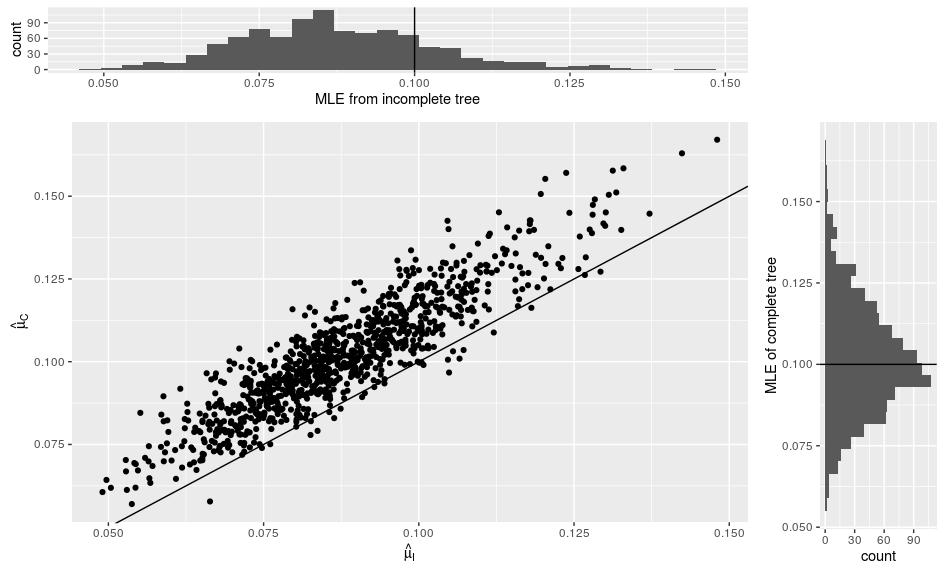
\includegraphics[width=\linewidth]{mu.png}
  %\caption{A really Awesome Image}\label{fig:awesome_image2}
\endminipage\hfill
\minipage{0.33\textwidth}%
  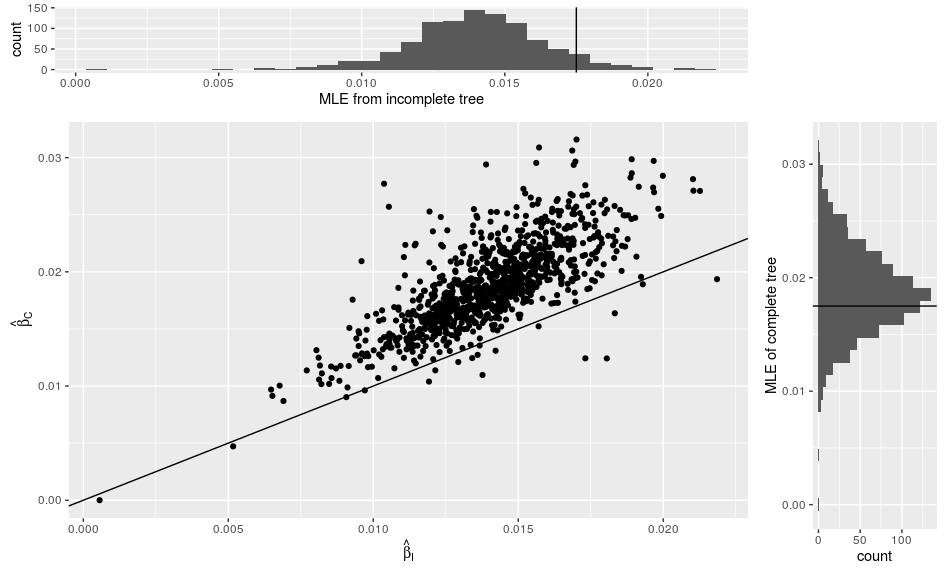
\includegraphics[width=\linewidth]{beta.png}
  %\caption{A really Awesome Image}\label{fig:awesome_image3}
\endminipage
\end{figure}

{\bf Analysis:} the reconstruction process is giving a good aproximation, however the aproximation is not enough in the sense that the new MLE is sligly biased which is an obstacle for the convergence of the EM algorithm. \\

The {\bf main reason} I see about why this aproximation is not unbiased is because from the observed tree we limite the framework to...



\section*{Solutions}

In order to obtain a robust method with convergence on the EM algorithm I see two posible ways with limited ideas to develope them 

\begin{itemize}

\item Continue with this aproximated algorithm described on previous section and find a way to compensate this underestimation of parameters. The problem with this option is that I do not see any way for that compensation yet. Do you have any idea?

\item Propose another reconstruction model wich use all information contained on the observed tree. A draft of a posible algorithm is described bellow.
\end{itemize}

\subsection*{An alternative algorithm}

%the function $P: \mathbb{N} \longrightarrow \mathbb{R}$ as
%\begin{equation}
%\begin{split}
%P(n)=  \displaystyle\int_{0}^{t_0}\displaystyle\int_{x_0}^{t_0}...\displaystyle\int_{x_{n-1}}^{t_0}\displaystyle\int_{x_n}^{t_0} e^{x_{\color{blue}{0}}(\lambda_{n+1}-\lambda_{\color{blue}{0}})}{\color{blue} \cdots} e^{x_{\color{blue}{n}}(\lambda_{n+1}-\lambda_{\color{blue}{n}})}\cdot\\
%\qquad \cdot[1-e^{-\mu_{\color{blue}{0}}(t_1-\sum_i^{{\color{blue}{0}}} x_i)}]{\color{blue} \cdots} [1-e^{-\mu_{\color{blue}{n}}(t_1-\sum_{i}^{{\color{blue}{n}}} x_i)}] dx_n dx_{n-1}...dx_1dx_0
%\end{split}
%\end{equation}


\end{document}